%! alt A circle with centre O and radius the square root of 425. Three chords pass through the point P inside it, at 60 degrees to each other, with lengths 32, 38 and 40. Their midpoints M1, M2 and M3 are the feet of the perpendiculars from O, at distances 13, 8 and 5 from O. The midpoints lie on the dashed circle with diameter OP and form an equilateral triangle, shaded, with O on the arc between M2 and M3.
%! after_paragraph 1
%! scale 1/5
%! let psi = 235
%! let b = asin(13/sqrt(172))*180/pi
% The shared preamble of every Cevian figure. pipeline/figures turns these colours into theme-aware paint,
% and refuses any other colour, so draw only with them:
%   figink (lines and labels), figaux (construction lines), figaccent (the object the argument turns on),
%   figtint and figaccenttint (light fills).
\documentclass[border=1.5pt]{standalone}
\usepackage{tkz-euclide}
\definecolor{figink}{RGB}{0,0,0}
\definecolor{figaux}{RGB}{85,85,85}
\definecolor{figaccent}{RGB}{192,57,43}
\definecolor{figtint}{RGB}{221,221,221}
\definecolor{figaccenttint}{RGB}{245,213,208}
% tkz-euclide's defaults draw circles, compasses and marks in 50% grey and fill points with a tint.
\makeatletter
\def\tkz@otherlinecolor{figink}
\def\tkz@euc@circlecolor{figink}
\def\tkz@euc@compasscolor{figink}
\def\tkz@euc@mkcolor{figink}
\def\tkz@mk@fill{figink}
\def\tkz@euc@pointfillcolor{figink}
\makeatother
\tkzSetUpLine[color=figink,line width=.7pt]
\tkzSetUpArc[color=figink,line width=.7pt]
\tkzSetUpCompass[color=figink,line width=.5pt]
\tkzSetUpPoint[color=figink,fill=figink,size=3.1pt]
\tikzset{
  every picture/.style={line cap=round,line join=round,color=figink},
  circle style/.append style={color=figink,line width=.7pt},
  aux/.style={color=figaux,line width=.45pt,dash pattern=on 2.6pt off 2pt},
  key/.style={color=figaccent,line width=1pt},
  mk/.style={color=figink,line width=.5pt},
  lbl/.style={color=figink,inner sep=2.2pt},
  len/.style={color=figink,inner sep=1.5pt,font=\small},
}

\begin{document}
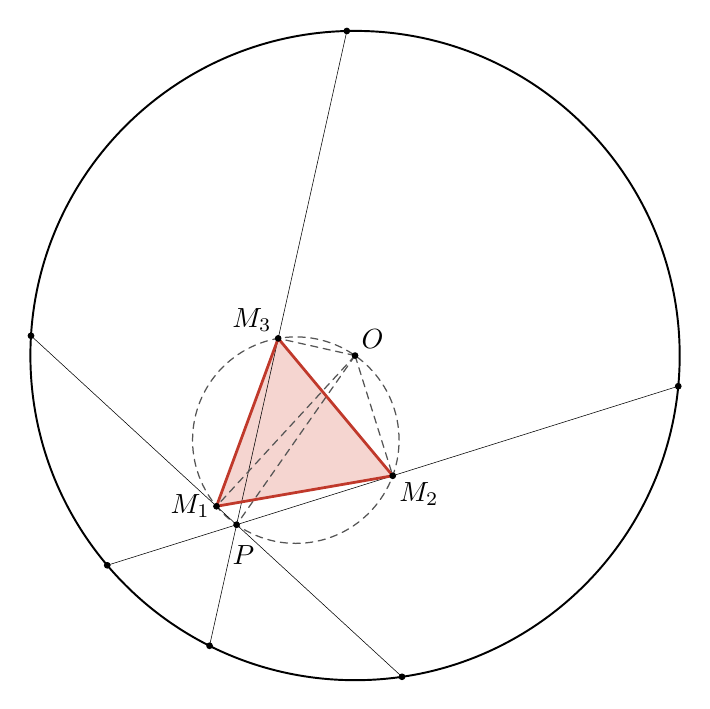
\begin{tikzpicture}
\tkzDefPoint(0.0,0.0){O} %! O = (0, 0)
\tkzDefPoint(-1.5044769,-2.1486157){P} %! P = polar(O, sqrt(172), psi)
\tkzDefPoint(-0.75223844,-1.0743078){W} %! W = mid(O, P)
\tkzDefPoint(-1.3572317,-2.2839628){Qa} %! Qa = polar(P, 1, psi + b)
\tkzDefPoint(-1.3136402,-2.0887712){Qb} %! Qb = polar(P, 1, psi + b + 60)
\tkzDefPoint(-1.4608854,-1.9534240){Qc} %! Qc = polar(P, 1, psi + b + 120)
\tkzDefPoint(-1.7595130,-1.9141875){Ma} %! Ma = foot(O, P, Qa)
\tkzDefPoint(0.47875600,-1.5266934){Mb} %! Mb = foot(O, P, Qb)
\tkzDefPoint(-0.97595828,0.21795740){Mc} %! Mc = foot(O, P, Qc)
\tkzDefPoint(0.59641005,-4.0797420){Xa} %! Xa = polar(Ma, 16, psi + b)
\tkzDefPoint(-4.1154361,0.25136700){Ya} %! Ya = polar(Ma, 16, psi + b + 180)
\tkzDefPoint(4.1046528,-0.38964789){Xb} %! Xb = polar(Mb, 19, psi + b + 60)
\tkzDefPoint(-3.1471408,-2.6637389){Yb} %! Yb = polar(Mb, 19, psi + b + 240)
\tkzDefPoint(-0.10412869,4.1217905){Xc} %! Xc = polar(Mc, 20, psi + b + 120)
\tkzDefPoint(-1.8477879,-3.6858757){Yc} %! Yc = polar(Mc, 20, psi + b + 300)
%! fact on_circle(Xa, O, sqrt(425))
%! fact on_circle(Ya, O, sqrt(425))
%! fact on_circle(Xb, O, sqrt(425))
%! fact on_circle(Yb, O, sqrt(425))
%! fact on_circle(Xc, O, sqrt(425))
%! fact on_circle(Yc, O, sqrt(425))
%! fact dist(Xa, Ya) == 32
%! fact dist(Xb, Yb) == 38
%! fact dist(Xc, Yc) == 40
%! fact collinear(P, Xa, Ya)
%! fact collinear(P, Xb, Yb)
%! fact collinear(P, Xc, Yc)
%! fact angle(Xa, P, Xb) == 60
%! fact angle(Xb, P, Xc) == 60
%! fact dist(O, Ma) == 13
%! fact dist(O, Mb) == 8
%! fact dist(O, Mc) == 5
%! fact concyclic(O, P, Ma, Mb, Mc)
%! fact dist(Ma, Mb) == sqrt(129)
%! fact dist(Mb, Mc) == sqrt(129)
%! fact dist(Mc, Ma) == sqrt(129)
%! fact angle(Mb, O, Mc) == 120
%! fact dist(O, P) == sqrt(172)
%! fact dist(P, Xa) * dist(P, Ya) == 253
\tkzFillPolygon[color=figaccenttint](Ma,Mb,Mc)
\tkzDrawCircle(O,Xa)
\tkzDrawCircle[aux](W,O)
\tkzDrawSegments(Xa,Ya Xb,Yb Xc,Yc)
\tkzDrawSegments[aux](O,Ma O,Mb O,Mc O,P)
\tkzDrawPolygon[key](Ma,Mb,Mc)
\tkzDrawPoints(O,P,Ma,Mb,Mc,Xa,Ya,Xb,Yb,Xc,Yc)
\tkzLabelPoint[above right,lbl](O){$O$}
\tkzLabelPoint[below=5pt,xshift=2.5pt,lbl](P){$P$}
\tkzLabelPoint[left,lbl](Ma){$M_1$}
\tkzLabelPoint[below right,lbl](Mb){$M_2$}
\tkzLabelPoint[above left,lbl](Mc){$M_3$}
\end{tikzpicture}
\end{document}
